\documentclass[12pt]{article}

\usepackage[a4paper,top=3cm,bottom=2cm,left=2cm,right=2cm,marginparwidth=1.2cm]{geometry}
\usepackage{fancyhdr}
\usepackage{graphicx}
\usepackage{float}
\usepackage{xcolor}
\usepackage{pgfplots}
\usepackage{caption}
\usepackage{mdframed}
\usepgfplotslibrary{fillbetween}
\pgfplotsset{compat=1.18}
\graphicspath{{./regressionPic/}}

\author{Eden Li}
\title{STAT110/115 Tutoring Materials – 02 Regression}
\date{}

\begin{document}
\pagestyle{fancy}
\lhead{STAT110/115 Tutoring Materials}
\rhead{Regression}
%\maketitle

\begin{itemize}
\item \textbf{Types of regression}: Linear (continuous data), Logistic (categorical data), Cox (categorical data in a survival analysis).
\item \textbf{Explanatory variable (X)}: Also known as a covariate, predictor, or independent variable.
\item \textbf{Outcome variable (Y)}: Also known as response or dependent variable.
\item \textbf{Simple Linear Regression (SLR)}: Looks at a relationship between two continuous variables where the relationship between the two variables is approximately a straight line.
\item \textbf{SLR equation}: $$Y = \beta_0 + \beta_1x + e$$
\begin{itemize}
\item This implies that the mean response is related to x by $$\mu_Y = \beta_0 + \beta_1x$$
\item \textbf{Y} is the numerical outcome variable (continuous or approximately so).
\item \textbf{x} is the explanatory variable.
\item \textbf{$\beta_0$} is the intercept or constant (where the line crosses the y-axis).
\item \textbf{$\beta_1$} is the slope of the line.
\item \textbf{e} (often denoted $\epsilon$) is the random error or residual term.
\end{itemize}
\item \textbf{SLR equation for estimating:}
$$\hat{y}=\hat{\beta}_0+\hat{\beta}_1x$$
\item \textbf{Residual ('estimated error') term}: $$\hat{e_i} = y_i - \hat{y_i}$$
\begin{figure}[H]
    \centering
    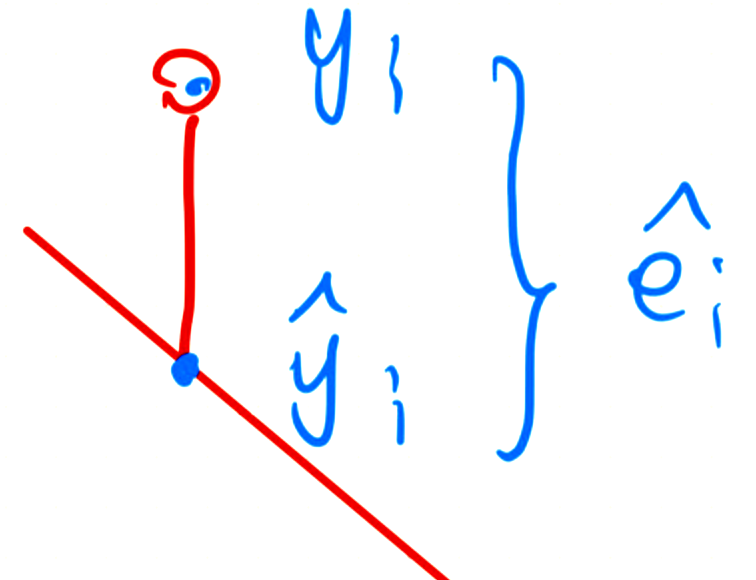
\includegraphics[width=0.2\textwidth]{92.png}
\end{figure}
\item \textbf{How to find regression line}: The line of best fit minimises the sum of the squares of the residuals.
\begin{figure}[H]
    \centering
    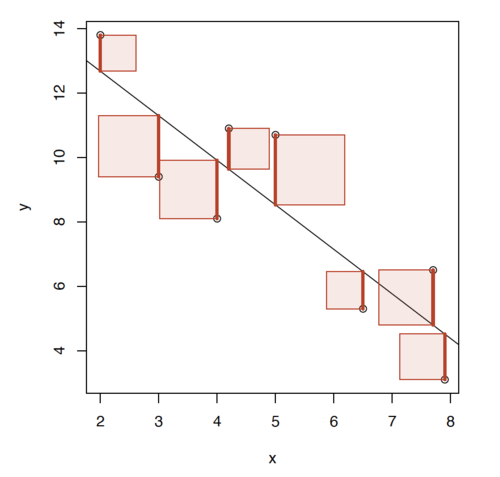
\includegraphics[width=0.3\textwidth]{1.png}
\end{figure}
\item \textbf{Equation for how to find regression line}:
$$\sum_{i=1}^{n}\hat{e}^2_i = \sum_{i=1}^{n}(y_i - \hat{y}_i )^2$$
\item \textbf{How to calculate $\beta_1$ and $\beta_0$}: 
$$\hat{\beta}_1 = \frac{\sum_{i=1}^{n}(x_i - \bar{x})(y_i - \bar{y})}{\sum_{i=1}^{n}(x_i - \bar{x})^2}$$
$$\hat{\beta}_0 = \bar{y} - \hat{\beta}_1 \bar{x}$$
\item \textbf{Example for how to calculate regression (Stress and Blood Pressure)}:
\begin{itemize}
\item Get n, n = 6
\item Find the explanatory and outcome 
\item Calculate $\beta_1$ and $\beta_0$
\item Get the regression equation
\item Using R for SLR
\end{itemize}
\item \textbf{Assumptions for Simple Linear Regression (LINE)}:
\begin{itemize}
\item Linearity: The relationship between the mean response $\mu_Y$ and x is described by a straight line.
\item Independence: The responses $Y_1,Y_2, . . . ,Y_n$ are statistically independent.
\item Normality: The error terms $e_1, e_2, . . . , e_n$ come from a normal distribution.
\item Equal variance: The error terms all have the same variance, $\sigma^2$ ('homoscedastic').
\end{itemize}
\item \textbf{What diagram is used for checking linearity}: Residual plot.
$$\hat{e}_i = y_i - \hat{y}_i = y_i - (\hat{\beta}_0 + \hat{\beta}_1 x_i) = y_i - \hat{\beta}_0 - \hat{\beta}_1 x_i$$
\item \textbf{Failure of linearity assumption}: 
\begin{figure}[H]
    \centering
    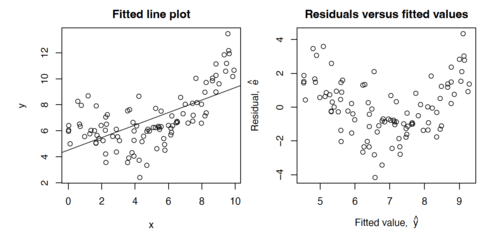
\includegraphics[width=0.7\textwidth]{2.png}
\end{figure}
\item \textbf{Linearity assumption holds}: 
\begin{figure}[H]
    \centering
    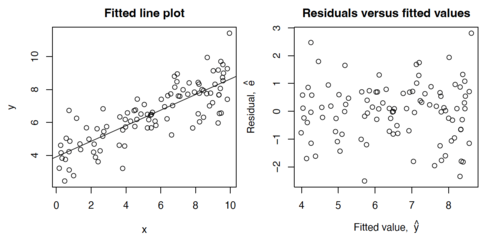
\includegraphics[width=0.7\textwidth]{3.png}
\end{figure}
\item \textbf{Checking independence assumption}: May get insight by thinking about the study design (Ask yourself questions).
\item \textbf{Plot for Checking the normality assumption}: Q - Q plot.
\item \textbf{Pass of normality assumption}: 
\begin{figure}[H]
    \centering
    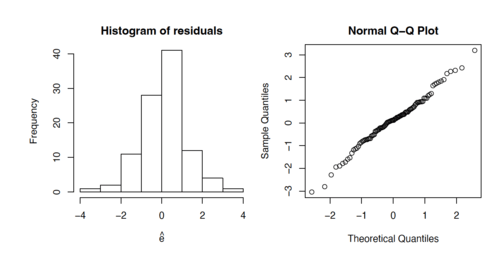
\includegraphics[width=0.7\textwidth]{4.png}
\end{figure}
\item \textbf{Fail of normality assumption}: 
\begin{figure}[H]
    \centering
    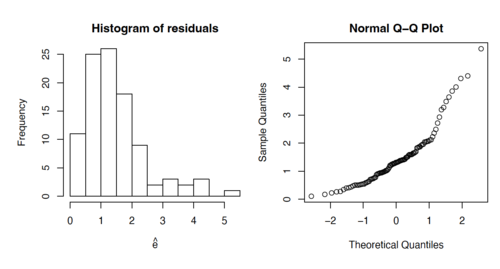
\includegraphics[width=0.7\textwidth]{5.png}
\end{figure}
\item \textbf{Checking equal variance assumption (homoscedasticity)}: Pass if the residual plot is not like this.
\begin{figure}[H]
    \centering
    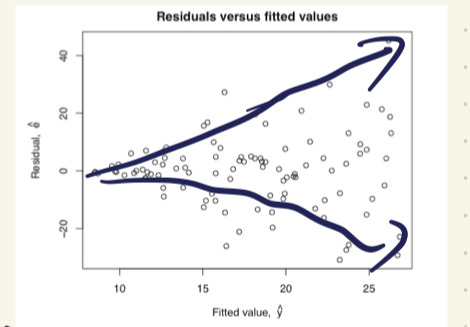
\includegraphics[width=0.5\textwidth]{6.jpg}
\end{figure}
\item \textbf{What is the impact if Fail of the linearity assumption}: Critical. If that assumption fails, all conclusions drawn from the model will be invalid.
\item \textbf{What is the impact if Fail of independence or equal variance assumptions}: Remain valid. However, estimates can be inefficient. Follows that the fitted regression line is useable. Any test results or confidence intervals based on the regression model will be invalid.
\item \textbf{What is the impact if Fail of normality assumption}: Typically least important. Effects validity of confidence intervals and test results when the sample size n is small.
\item \textbf{What to do with outliers}: The first thing to do is check that the data are correctly recorded. If data cannot be corrected, try refitting regression with outliers removed, but still investigate the cause of outliers - may be very important.
\item \textbf{Estimate of error variance}: 
$$S^2_e = \frac{1}{n-2}\sum_{i=1}^{n}(\hat{e}^2_i)=\frac{RSS}{n-2}$$
$$where \ RSS = \sum_{i=1}^{n}\hat{e}^2_i \ is \ the \ residual \ sum \ of \ squares.$$
\item \textbf{Degree of freedom for SLR's CI}: v = n - 2 because there're two parameters.
\item \textbf{What is the multiplier for SLR's CI}: 
$$t = \frac{estimate - null}{std. error}$$
\item \textbf{What is the SE for SLR's CI}:
$$s_{\hat{\beta}_1} = \frac{s_e}{\sqrt{\sum_{i=1}^{n}(x_i - \bar{x})^2}}$$
\item \textbf{Using R to find SLR's CI}: 
\begin{mdframed}[backgroundcolor=gray!15, linecolor=black]
\begin{verbatim}
> confint(model1)
                 2.5 %     97.5 %
(Intercept) 24.8300345 62.4009555
X            0.2557407  0.7284774
\end{verbatim}
\end{mdframed}
\item \textbf{$\beta_1 = 0$ indicates what}: That the response is not (linearly) related to the predictor. So the estimated slope will (almost) always be non-zero: $\hat{\beta_1} \neq 0$.
\item \textbf{Steps to test to assess the strength of evidence in the data for $\beta_1 \neq 0$}:
\begin{itemize}
\item Setting up the hypotheses: $H_0 : \beta_1 = 0$, $H_A : \beta_1 \neq 0$.
\item Calculating The test statistic
$$t = \frac{\hat{\beta}_1}{s_{\hat{\beta}_1}}$$
\item Computing the p-value
\item Draw conclusion with rejecting or not $H_0$
\end{itemize}
\item \textbf{When predicting the data}: Ignore $e_0$.
\item \textbf{Why not recommend extrapolating when predicting data}: The plot may not be linear.
\begin{figure}[H]
    \centering
    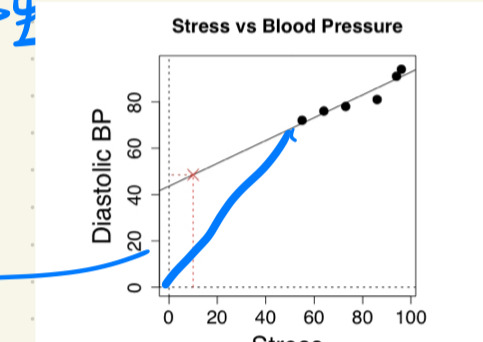
\includegraphics[width=0.4\textwidth]{7.jpg}
\end{figure}
\item \textbf{Prediction error}: The prediction error is analogous to a standard error, but takes account of both sources of uncertainty. For prediction at $x_0$, the prediction error is: 
$$PE(\hat{y}_0) = s_e\sqrt{1 + \frac{1}{n} + \frac{(x_0 - \bar{x})^2}{\sum_{i=1}^{n}(x_i - \bar{x})^2}}$$
\item \textbf{Prediction interval formula}:
$$\hat{y}_0 \pm t_{(1-\frac{\alpha}{2}, n-2)} \times PE(\hat{y}_0)$$
\item \textbf{Correlation coefficient (r)}: Summarises the strength of a linear relationship between variables. It is a measure of linear association between variables. It describes both the strength and direction of the relationship.
$$r = \frac{\sum_{i=1}^{n} (x_i - \bar{x})(y_i - \bar{y})}{\sqrt{\sum_{i=1}^{n}(x_i - \bar{x})^2 \sum_{i=1}^{n}(y_i - \bar{y})^2}}$$
\begin{itemize}
\item \textbf{r} $\in [-1, 1]$. A positive value of r means that Y and X increase together. A negative value of r means that as X increases, Y decreases (and vice-versa). 
\item The strength of the linear relationship increases as r tends towards 1 or -1. r = 0 corresponds to no linear relationship between the variables.
\end{itemize}
\item \textbf{Scatterplots for r}: 
\begin{figure}[H]
    \centering
    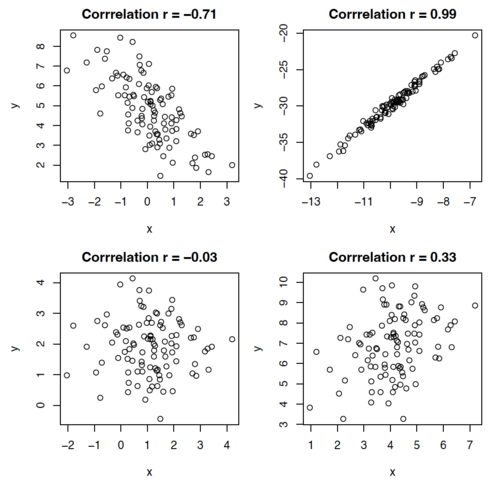
\includegraphics[width=0.7\textwidth]{8.png}
\end{figure}
\item \textbf{Re-write for r}: $s_x$ and $s_y$ are sample standard deviations for x and y variables. $s_{xy}$ is the sample covariance between x and y.
$$= \frac{S_{xy}}{S_x S_y}$$
\item \textbf{Correlation coefficient versus regression models}: The correlation coefficient is a summary of the data. Unlike linear regression, the correlation coefficient does not specify a model for the data, and cannot (for example) be used for prediction. The correlation coefficient is symmetric in the variables. That is, the correlation between x and y is the same as the correlation between y and x. In regression, the variables are not handled symmetrically. Regression models look at variation in Y for fixed values of x.
\item \textbf{Coefficient of determination ($R^2$)}: $R^2$, is a measure of how well a regression model describes the data. $R^2$ is the squared correlation between the observed and predicted responses. $R^2 \in [0, 1]$.
\item \textbf{Meaning for the value of $R^2$}: A high value of $R^2$ (close to 1) indicates a regression model that describes the data very well. Conversely, a low value of $R^2$ (close to 0) indicates a regression that describes the data poorly.
\begin{figure}[H]
    \centering
    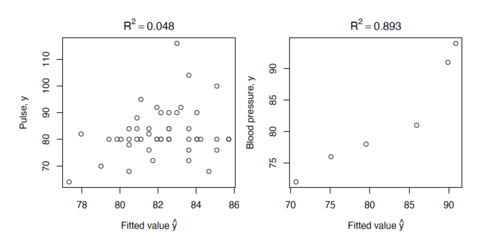
\includegraphics[width=0.7\textwidth]{9.png}
\end{figure}
\item \textbf{What describes the overall variation in the response variable?}: Total sum of squares.
$$TSS = \sum_{i=1}^{n} (y_i - \bar{y})^2$$
\item \textbf{What describes the total variation of the data points about the regression line?}: Residual sum of squares (RSS can be thought of as variation not explained by the regression model).
$$RSS = \sum_{i=1}^{n} (y_i - \hat{y}_i)^2$$
\item \textbf{What describes as the amount of variation in the response that is explained by the regression model?}: Explained sum of squares.
$$ESS = TSS - RSS$$
\item \textbf{Equation of $R^2$}: 
$$R^2 = \frac{ESS}{TSS} = 1 - \frac{RSS}{TSS}$$
\item \textbf{Correlation does not equal causation}: e.g., just because there's more ice cream in the summer and more drowning in the summer doesn't mean there's a link between ice cream and drowning.
\item \textbf{Logistic regression}: Outcome variable is binary.
\begin{figure}[H]
    \centering
    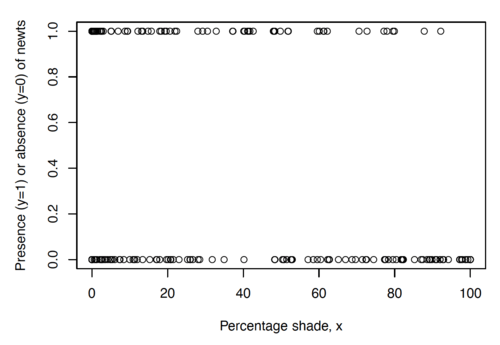
\includegraphics[width=0.5\textwidth]{91.png}
\end{figure}
\item \textbf{Equation for logistic regression}: 
$$logit(p) = \log\left(\frac{p}{1-p}\right) = \beta_0 + \beta_1x$$
$Y$ is the binary outcome variable, $Y = 1$ or $Y = 0$ for each observation. $p$ is the probability that specified category will occur; i.e. $p = Pr(Y = 1)$. $x$ is the explanatory variable. Parameters $\beta_0$, $\beta_1$ are the regression coefficients. $\beta_0$ is intercept and $\beta_1$ slope 'on the logit scale'. In the formula, log is the natural logarithm (log to base e).
\item \textbf{Which technique do we use when estimating the regression coefficients?}: Maximum likelihood estimation.
\item \textbf{What will increase x by one unit result in?}: A multiplicative change of $e^{\beta_1}$ to the odds.
\item \textbf{Formula for logistic curve for the probability p}: 
$$p = \frac{e^{\beta_0 + \beta_1x}}{1+e^{\beta_0 + \beta_1x}}$$
\item \textbf{Testing in logistic regression}:
\begin{itemize}
\item Define the hypotheses: $H_0 : \beta_1 = 0$ and $H_A : \beta_1 \neq 0$.
\item The test statistic is: 
$$z = x\frac{\hat{\beta}_1}{s_{\hat{\beta}_1}}$$
\item Get the corresponding p-value.
\item Reject/not reject $H_0$.
\item Conclusion.
\end{itemize}
\item \textbf{Multiple regression model}:
$$Y = \beta_0 + \beta_1x_1 + \cdots + \beta_kx_k + e$$
\item \textbf{Mean value of the Multiple regression model}: 
$$\mu_Y = \beta_0 + \beta_1x_{1} + \cdots + \beta_kx_{k}$$
\item \textbf{Applications of multiple regression}:
\begin{itemize}
\item Adjusting for the effect of confounding variables.
\item Establishing which variables are important in explaining the values of the response variable.
\item Predicting values of the response variable.
\item Describing the strength of the association between the response variable and the explanatory variables.
\end{itemize}
\item \textbf{Least squares estimates}: 
$$\sum_{i=1}^{n} (y_i - \hat{y}_i)^2$$
\item \textbf{RSS for $\hat{e_i}$}: 
$$RSS = \sum_{i=1}^{n} \hat{e}_i^2$$
To estimate the error variance $\sigma^2_e$.
\item \textbf{Usual estimate}: 
$$s_e^2 = \frac{RSS}{n - k - 1}$$
\end{itemize}

\end{document}
